\documentclass[a4j]{jarticle}
    \usepackage[dvipdfmx]{graphicx}
    \usepackage[ top=25truemm,bottom=25truemm,left=25truemm,right=25truemm]
    {geometry}
    \usepackage{ascmac}
    \usepackage{array}
    \usepackage{here}
    \usepackage{url}
    \usepackage{listings, jlisting}
    \renewcommand{\lstlistingname}{リスト}
\lstset{language=c,
  basicstyle=\ttfamily\scriptsize,
  commentstyle=\textit,
  classoffset=1,
  keywordstyle=\bfseries,
  frame=tRBl,
  framesep=5pt,
  showstringspaces=false,
  numbers=left,
  stepnumber=1,
  numberstyle=\tiny,
  tabsize=4
}

\makeatletter
\def\@thesis{プログラミング演習 レポート}
\def\id#1{\def\@id{#1}}
\def\department#1{\def\@department{#1}}

\def\@maketitle{
\begin{center}
{\huge \@thesis \par} %修士論文と記載される部分
\vspace{10mm}
{\LARGE\bf \@title \par}% 論文のタイトル部分
\vspace{10mm}
{\Large \@date\par}	% 提出年月日部分
\vspace{20mm}
{\Large \@department \par}	% 所属部分
{\Large 学籍番号 \@id \par}	% 学籍番号部分
\vspace{10mm}
{\Large 氏名 \@author}% 氏名 
\end{center}
\par\vskip 1.5em
}

\title{ミニゲーム}
\date{提出期限 2021年1月18日 17:00}
\department{組番号 408}
\id{17406}
\author{金澤雄大}

    \begin{document}
    \maketitle
    \thispagestyle{empty}
    \clearpage
    \addtocounter{page}{-1}
    \section{目的}
    後期のプログラミング演習で学習した内容の理解度を高めるために,ミニゲームを作成することを目的とする.
    \section{ミニゲームの説明}
    本章では,ゲームの概要,用語,設定,仕様の4つについて述べる.
    \subsection{ゲームの概要}
    ミニゲームとして,「桃太郎電鉄」\cite{mmtt}(以下,桃鉄)をイメージした「ちゃま鉄」を作成した.「ちゃま鉄」は鉄道会社の運営をイメージしたすごろく形式のゲームである.
    本ゲームは,3年決戦で3人でのプレイを想定しており,CPUキャラは存在しない.また桃鉄における「貧乏神」,「すりの銀次」,「臨時収入」を代表とする要素は開発時間の都合上実装していない.
    \subsection{プレイヤーと物件の設定}
    プレイヤーおよび物件の設定について説明する.先述した通り,プレイヤー(社長と呼ぶ)は3人おり,ゲーム内ではターン順に「プレイヤー1社長」,「プレイヤー2社長」,「プレイヤー3社長」と
    呼ばれる仕様になっている.さらに各社長には色の設定が行われている.社長名と色の対応を次に示す.
    \begin{itemize}
        \item プレイヤー1社長 $\cdots$ 青
        \item プレイヤー2社長 $\cdots$ ピンク
        \item プレイヤー3社長 $\cdots$ 黄色
      \end{itemize}
       各社長には「所持金」,「総資産」という2つのパラメータが割り振られている.ゲームスタート時の所持金は1億円,総資産は0円である.所持金は社長が手元に持っているお金のことである.停車する駅には
      「物件」を購入できる「物件駅」というものがあり,この物件を購入することで総資産を増やすことができる.図\ref{bukkenex}に長野駅の物件の例を示す.
      図\ref{bukkenex}には6つの物件がある.物件には「価格」,「収益率」という2つのパラメータがある.例えば「りんごえん」の場合,価格が「600万円」,収益率が「120\%」である.
      価格はその物件を購入するために必要な所持金であり,収益率は決算(後述)で手に入るお金の割合を示している.また,同じ駅の物件を1人の社長がすべて購入すると「独占」という
      状態になる.独占状態になった駅の収益率は2倍になり,決算で2倍の収益が得られる仕様になっている.

      \begin{figure}[H]
        \centering
        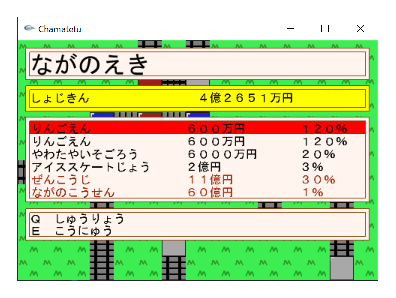
\includegraphics[scale=1.5]{bukkenex.eps}
        \caption{物件の例(長野駅)}
         \label{bukkenex}
        \end{figure}
    
    \subsection{ゲームの進行方法}
    ゲームの進行について説明する.ここではゲームの進行の概要について説明し,実際の画面表示については実装部分と共に述べる.
    図\ref{processgame}にゲーム進行のフローチャートを示す.ゲームを開始すると,初期設定が行われ,タイトル画面が表示される.
    初期設定としてはゲームスタート時の駅の設定および年月の設定が行われる.ゲームスタート時の駅は長野駅,年月は「1年目4月」に設定が行われる仕様にした.
    次に目的地の設定が行われる.目的地の処理の詳細については!で述べる.目的地の設定が完了するとゲームのメイン部分である社長の行動が始まる.各社長はターン中に
    サイコロを1つふって出た目の数だけ進む,もしくはカードを使う,のどちらかの行動を行うことができる.各社長が1回行動すると,年月の経過処理として1ヵ月経過する処理が行われる.
    年月の経過処理後の処理は月によって変化する.3月でない場合は再び社長の行動の処理が行われる.3月の場合は社長の行動の前に「決算」という処理が行われる.決算の処理については!で述べる.
    さらに3年目の場合は決算として最終成績が表示されゲームの終了処理が行われる.
    \begin{figure}[H]
        \centering
        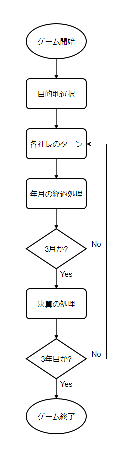
\includegraphics[scale=2.3]{processgame.eps}
        \caption{ゲームの進行}
         \label{processgame}
        \end{figure}

    \subsection{マップの設定}
    マップの設定について説明する.図\ref{map}に本ゲームのマップを示す.図\ref{map}の地名からも読み取れるように,本ゲームは長野県を舞台にしている.
    ただし,実際のゲームでは駅名は表示されない仕様になっている.マップは32$\times$32の画像を敷き詰める形で描画しており,サイズは960$\times$960である.
    なお,ウィンドウサイズは幅480,高さ320のため実際のゲームでは,行動中の社長を中心として画面におさまる部分だけを描画している.

    \begin{figure}[H]
        \centering
        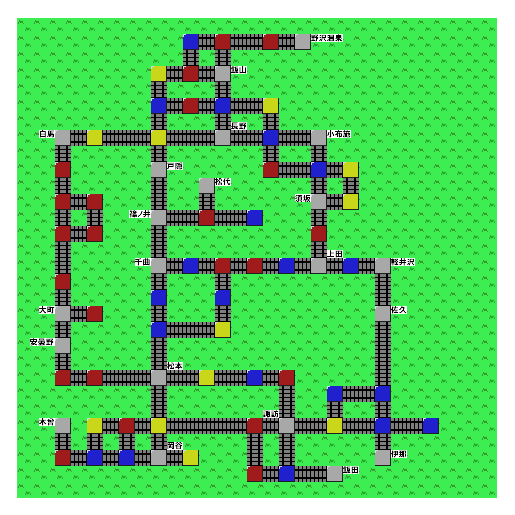
\includegraphics[scale=1.9]{map.eps}
        \caption{ゲームのマップ}
         \label{map}
        \end{figure}

    マップを描画する画像には表\ref{mapimage}に示す種類のものがある.
    これらの画像は「/mapparts」に保存されている.背景は季節によって変化する.月と季節は次に示すようになっている.図\ref{map}の
    マップは背景が春の場合である.季節ごとに背景が変化する仕様は桃鉄を参考にした.
    \begin{itemize}
        \item 春 : 3月~5月 
        \item 夏 : 6月~8月 
        \item 秋 : 9月~11月 
        \item 冬 : 12月~2月 
      \end{itemize}

\begin{table}[H]
  \caption{マップとして描画される画像の種類}
\label{mapimage}
\begin{center}
    \begin{tabular}{c|c|c}\hline
        画像の意味 & 画像のファイル名 & 実際の色や模様 \\ \hline \hline
        背景(春) & season1.png & 明るい緑 \\ 
        背景(夏) & season2.png & 濃い緑 \\
        背景(秋) & season3.png & 茶色 \\
        背景(冬) & season4.png & 白 \\
        プラス駅 & map1.png & 青 \\
        マイナス駅 & map2.png & 赤 \\
        カード駅 & map3.png & 黄色 \\
        物件駅 & map4.png & 灰色 \\ 
        線路(縦) & map5.png & 灰色背景に黒の線路 \\ 
        線路(横) & map6.png & 灰色背景に黒の線路 \\ 
        目的地駅 & map7.png & 灰色背景に駅のマーク\\ \hline
    \end{tabular}
\end{center}
\end{table}

    \subsection{駅の設定}
    駅の設定について説明する.サイコロをふって移動した社長が停車できる駅の種類には,表\ref{mapimage}に示したように,「プラス駅」,「マイナス駅」,「カード駅」,「物件駅」,「目的地駅」の5つがある.
    プラス駅は停車するとお金がもらえる駅である.もらえるお金は夏が最も多く,冬が最も少ない仕様になっている.マイナス駅は停車すると所持金が減少する駅である.
    減少する金額は夏が最も少なく,冬が最も多い仕様になっている.減少する額によっては所持金が負になる,いわゆる借金という状態になることがある.この場合,
    物件を売却することで借金を返済する処理が行われる.本ゲームでの借金の返済は売却する物件を選択する方式ではなく,自動で売却する物件を選ぶ方式を採用した.
    売却する物件の優先順位は次に示す通りである.なお,所持している全ての物件を売却しても借金が返済できない場合は所持金が負となった状態でターンが終了する.
    \begin{enumerate}
        \item 独占している駅の物件でなく,借金額よりも価格が高い物件
        \item 独占している駅の物件でなく,借金額よりも価格が低い物件
        \item 独占している物件で,借金額よりも価格が高い物件
        \item 独占している物件で,借金額よりも価格が低い物件
    \end{enumerate}
     カード駅は停車するとカードがもらえる駅である.カードは5枚まで所持することができ,カード駅に停車したときに既に5枚カードを持っている場合,この処理はスキップされる.
    カードは表\ref{cardlist}に示す8種類がある.カード名は桃鉄を参考にした.表\ref{cardlist}のカードのうち,急行カード,特急カード,新幹線カードの3種類は
    カードを仕様したあとにサイコロをふって移動することができる.他のカードについは,成功,失敗にかかわらずターンが終了する.
    \begin{table}[H]
        \caption{カード名と効果}
      \label{cardlist}
      \begin{center}
          \begin{tabular}{c|c}\hline
              カード名 & カードの効果 \\ \hline \hline
              急行カード & サイコロが2個に増える.\\
              特急カード & サイコロが3個に増える.\\
              新幹線カード & サイコロが4個に増える.\\
              サミットカード & すべての社長を自分のマスに集める.3分の2の確率で成功する.\\
              ぶっとびカード & ランダムな物件駅に移動する. \\
              10億円カード & 10億円が手に入る.\\
              徳政令カード & 借金を負っている社長の所持金が0円になる.\\
              剛速球カード & 他の社長のカードをすべて破棄する.2分の1の確率で成功する.\\ \hline
          \end{tabular}
      \end{center}
      \end{table}

      \subsection{決算の処理}
      決算の処理について説明する.決算は3月が終了すると行われる処理である.決算は,所持している物件に応じて各社長の所持金が
      増加する処理である.ある社長が決算で得られる金額$S$を計算する方法について説明する.物件を$n$個持っており,所持している$i$番目の物件の価格$p_i$,
      収益率$r_i$,その物件が所属する駅が自分の独占のとき$d_i=2$,独占でないとき$d_i=1$とする.このとき,決算で得られる金額$S$は式(\ref{kessan})で表せる.
      \begin{equation}
        S = \sum_{i=1}^{n} \frac{p_i r_i d_i}{100}
        \label{kessan}
      \end{equation}
      例えば,ある社長が,図\ref{bukkenex}の「やわたやいそごろう」と「アイススケートじょう」を所持している場合に
      決算でもらえる金額を計算してみる.式(\ref{kessan})に値を代入して計算を行うと,式(\ref{kessan_ex1})に示すように1800万円になる.
      この例では独占はしていないから$d_i$は常に1である.

      \begin{eqnarray}
        S &=& \sum_{i=1}^{n} \frac{p_i r_i d_i}{100} \\
          &=& \frac{1}{100} \left( 6000\times10^4 \cdot 20 + 20000\times10^4 \cdot 3 \right) \\
          &=& 1800 \times10^4
        \label{kessan_ex1}
      \end{eqnarray}    
       本ゲームは3年決戦であるため,3年目の決算は「最終成績」という形で表示される.最終成績を表示した後はゲームを終了するように促す画面を表示する.
    
      \section{実行環境とビルド方法}
      本章では,実行環境,ビルド方法,ディレクトリ構造の3つについて述べる.
      \subsection{実行環境}
      実行環境を\ref{env}に示す.gccとは「GNU Compiler Collection」の略称で,GNUプロジェクトが公開しているコンパイラのことである.
      makeはMakefileにプログラムのコンパイルやリンクの方法を指示することで,コンパイルを簡単に行うことができるツールのことである.
      makeを用いることは,gccコンパイル時に,長いオプションを入力しなくてよい,ファイルの更新を取得して必要なものだけをコンパイルしてくれる
      という利点がある.
      
      \begin{table}[H]
        \caption{実行環境}
      \label{env}
      \begin{center}
          \begin{tabular}{c|l}\hline
            CPU & Intel(R) Core(TM) i7-6500U 2.50GHz  \\ 
            メモリ & 16.0GB DDR4 \\
            OS & Microsoft Windows 10 Home \\
            gcc &  version 9.3.0 \\
            make & version 4.3 \\ \hline
          \end{tabular}
      \end{center}
      \end{table}
      
      \subsection{ビルド方法}
      ビルド方法について説明する.まず,「j17406.tar.gz」を保存したディレクトリに移動する.次にリスト\ref{kaito}に示すコマンドを実行する.
      リスト\ref{kaito}
      \begin{lstlisting}[basicstyle=\ttfamily\footnotesize, frame=single,label=kaito,caption=j17406.tar.gzの解凍]
gzip -dv j17406.tar.gz
tar xvf j17406.tar
        \end{lstlisting}
      
      \subsection{ディレクトリ構造}

    \begin{thebibliography}{9}
        \bibitem{mmtt}  桃太郎電鉄,\url{https://www.konami.com/games/momotetsu/teiban/} ,閲覧日2021年1月5日
        \end{thebibliography}
\end{document}

